\documentclass[12pt]{article}
\usepackage[english]{babel}
\usepackage{amsmath}
\usepackage{amssymb}
\usepackage{amsmath, amssymb}
\usepackage{bm}
\usepackage{graphicx}
\usepackage[printonlyused]{acronym}
\usepackage{color}
\usepackage{listings}

\usepackage[colorinlistoftodos,prependcaption,textsize=tiny]{todonotes} % great for keeping track of todos
\usepackage{xargs}                      % Use more than one optional parameter in a new commands
\usepackage{xcolor}  % Coloured text etc.
\newcommandx{\info}[2][1=]{\todo[linecolor=green,backgroundcolor=green!25,bordercolor=green,#1]{\textbf{Info:} #2}}
\newcommandx{\toadd}[2][1=]{\todo[linecolor=blue,backgroundcolor=blue!25,bordercolor=blue,#1]{\textbf{To-add:} #2}}
\newcommandx{\change}[2][1=]{\todo[linecolor=yellow,backgroundcolor=yellow!25,bordercolor=yellow,#1]{\textbf{Change:} #2}}
\newcommandx{\error}[2][1=]{\todo[linecolor=red,backgroundcolor=red!25,bordercolor=red,#1]{#2}}

\title{Application of Gaussian Process regression to the Estimation of time-in-therapeutic-range (TTR) and prediction of the international normalized ratio (INR) in patients under therapy with Vitamin K antagonists}
\author{Franz Ruderich}


\begin{document}
	\maketitle
	
	\clearpage
	
	\bibliographystyle{unsrt}
	
	\tableofcontents
	
	\clearpage
		
	\section{Background}
	\graphicspath{{background/}}
	The \ac{TTR} is an important measure for the effectivity of many pharmacological therapies. \ac{TTR} describes the time in which a patient during a drug treatment has an effective mirror in target range. In this range the patient will experience the desired clinical effect with a minimum of undesirable adverse drug reactions. 

Coumarine derivates are a group of drugs with a similiar structure like Vitamine K. They interfere with the metabolism of Vitamine K as competetive \ac{VKA}. \ac{VKA} inhibit the Vitamine K dependent $\gamma$-carboxilation of the blood clotting factors II, VII, IX and X in the liver. As a result the clotting factors become inactive and blood clotting is delayed. The reduction of the blood coagulation is measured by the \ac{INR} \cite{Hirsh_1998}. The most important coumarines in human medicine used \ac{VKA} are Phenprocoumon and Warfarine. They are used to prevent intravasal thrombembolism. Patients suffer from chronic atrial fibrilation are at high risk to get thrombembolisms in the atrium of the heart and incur a stroke. The livelong therapy with \ac{VKA} reduce the risk of these complications.

But the required therapeutic dosage of \ac{VKA} has a large interindividual variability. Reasons for this phenomen are that the enzymes, responsible for the metabolism of \ac{VKA}, are highly polymorph \cite{Brehm_2016,  Verhoef_2014}. In addition depends the effectiveness of coumarin derivates on the resorption amd metabolism of the single patient. Many drugs and food interact with the metabolism of \ac{VKA} resulting in an intraindividual day-to-day variability of anticoagulative effect. Figure \ref{inr_panel} shows the variability of   

\begin{figure}
	\centering
	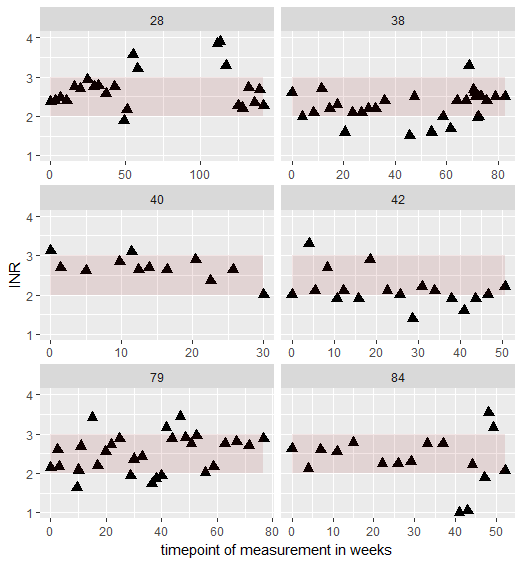
\includegraphics{./images/inr_panel.png}
	\label{inr_panel}
	\caption{Typical INR-Values over time. Lightred area is the therapeutic range}
\end{figure}

    
Two popular methods for therapeutic control of anticoagulation 
Time in therapeutic range assesed by linear interpolation of successive INR measurements
Cross-sectional proportion of all patients' last INR in therapeutic Range

	
	\clearpage
	\graphicspath{{existing_work/}}
	\section{Existing work}
	Oral anticoagulation has been shown to prevent thrombembolism efficiently for several indications.  However the precondition is that the inhibition of clotting, measured by \ac{INR}, is between close borders. To weak inhibition is associated with the risk of thrombembolic events, to strong inhibition increases the risk of gastrointestinal or cerebral bleedings \cite{Van_der_Meer_1993}.

Measurement of INR at fixed intervals and calculating the time in therapeutic range is necessary to protect patients under therapy with \ac{VKA} from complications.

In studies and daily clinical work \ac{TTR} is be calculated by different methods \cite{Kaatz_2008}:


The simplest method calculates the percentage of \ac{INR} within the therapeutic range \ac{PINRR}. The \ac{PINRR} method counts how many measurements had INR results in range. This number is divided by the total numbers of visits. For the data of patient depicted in figure \ref{example_patient} 18 of 26 values are in range. So the estimation for time in therapeutic range is $\frac{18}{26}= 69 \%$. 

\begin{tabular}{l*{8}{c}}
	tp& 
	0 & 3 & 6.7 & 10.7 & 15.7 & 19.7 & 24.7 & 29 \\
	inr&
	\colorbox{green}{2.37}&
	\colorbox{green}{2.41}&
	\colorbox{green}{2.47}&
	\colorbox{green}{2.41}&
	\colorbox{green}{2.76}&
	\colorbox{green}{2.70}&
	\colorbox{green}{2.93}&
	\colorbox{green}{2.75}\\
	tp&
	32 & 37 & 42.7 & 48.9 & 51 & 55 & 57 & 58 \\
	inr&
	\colorbox{green}{2.79}&
	\colorbox{green}{2.58}&
	\colorbox{green}{2.76}&
	\colorbox{red}{1.89}&
	\colorbox{green}{2.16}&
	\colorbox{red}{3.56}&
	\colorbox{red}{4.45}&
	\colorbox{red}{3.21} \\
	tp&
	111.1&112.9&116.9&120.9&124.9&127.9&131.9&135.9 \\
	inr&
	\colorbox{red}{3.85}&
	\colorbox{red}{3.89}&
	\colorbox{red}{3.28}&
	\colorbox{red}{4.10}&
	\colorbox{green}{2.28}&
	\colorbox{green}{2.21}&
	\colorbox{green}{2.72}&
	\colorbox{green}{2.35} \\
	tp&
	139.3 & 141.9\\
	inr&
	\colorbox{green}{2.67}&
	\colorbox{green}{2.27}
	
\end{tabular}


\begin{figure}
	\centering
	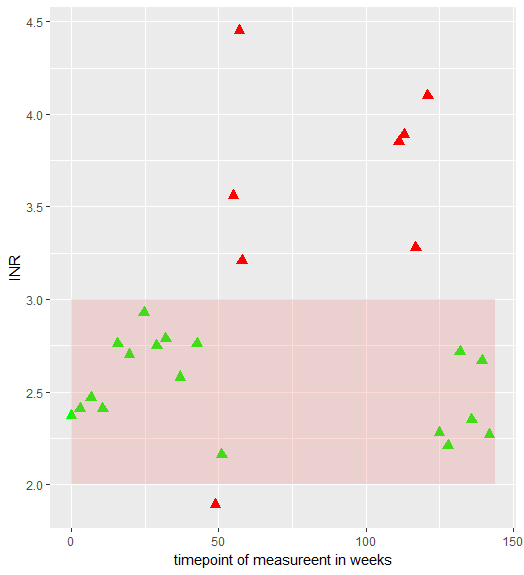
\includegraphics{inr_scatterplot.png}
	\label{example_patient}
	\caption{INR values over time of a single example patient. Green points are values in range, red points values out of range} 
\end{figure}

The more complex method of calculation \ac{TTR} is the so called "Rosendaal method" \cite{Rosendaal_1993}. It has become the mostly used method of determing how well a patient is maintaining his \ac{INR} test results in clinical studies. This method measures percantage time in\ac{TTR} using linear interpolation. The underlying assumption is that the \ac{INR} value between two measurements vary in a linear manner from the first to second value. 

One possibility to calculate \ac{TTR} is to divide the time between two measurements in  halves and allocate the first halve to the first \ac{INR} and second halve to second \ac{INR}.

The more distinguished possibility assumes that changes between consecutive \ac{INR} are linear over time and takes account of the steepness of change of inr-values between measurements. Calculating \ac{TTR} by "Rosendaal-Method" is more difficult when one measurement is within the therapeutic range and the second is out. The part of time in \ac{TTR} is the calculated by

\begin{align}
	\frac{\text{difference of inr in range}}{\text{difference of inr}} * {\text{difference of time}}
\end{align} 

For example at timepoint 51 the inr value is 2.16 in range. At the next timepoint 55 the inr value is 3.56 out of therapeutic range. 
The part of time in therapeutic range between the two measurements is calculated by

\begin{align} 
\text{time in therapeutic range} = \frac{3-2.16}{3.56-2.16}*(55-51)=\frac{0.84}{1.4}*4=3
\end{align}. 

So it is assumed that 3 weeks of the 5 weeks between the two measurements the \ac{INR} was in therapeutic range an two weeks out of it. 

Calculating the \ac{TTR} for the example patient shows, that the \ac{INR} was 83.5\% of time in therapeutic range.   
     
One problem with the Rosendaal linear extrapolation method is that it is unknown whether the \ac{INR} really varies linear between measurements. The linear model is a simplification because the real shape of the \ac{INR} course is unknown. But linear interpolation may not account for dose changes that are not followed shortly thereafter by repeat \ac{INR} testing (figure \ref{rosendaal_examples}).

\begin{figure}
	\centering
	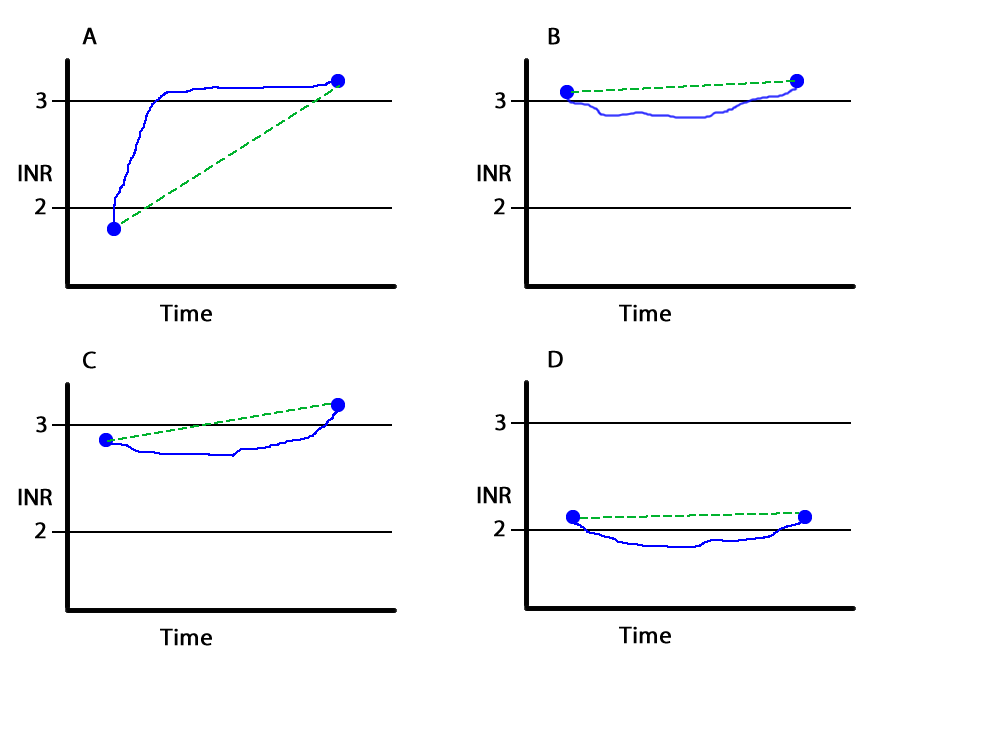
\includegraphics{rosendaal_examples.png}
	\label{rosendaal_examples}
	\caption{Examples of misevaluation  of \ac{INR} course (blue line) by linear interpolation (dotted line) between \ac{INR} measurements (blue points) 
	A: Both \ac{INR} values are out of range. The INR raises fast, but the lineaar interpolation overestimates \ac{TTR}. B: Both \ac{INR} measurements are hardly out of range, but the \ac{INR} course is in range. The \ac{TTR} is underestimated. C: One \ac{INR} is in range, the second out. The \ac{INR} course is in range most of the time. The \ac{TTR} is underestimated by linear interpolation. D: Both \ac{INR} values are in range. The \ac{INR} course is under the range most of the time. The \ac{TTR} is overestimated by linear interpolation.}
\end{figure}


	
	\graphicspath{{data_and_methods/}}
	\section{Data and methods}
	\subsection{Gaussian Processes for Regression}
	For noisy measurements of (laboratory) values at certain time points it is difficult to fix
	what the best estimates of values between the time points or at future time points are.
	The assumption of an underlying linear function makes it easy to fit a straight line by least-squares method. But this is often a oversimplification of the problem. The model will provide poor predictions, if the relationship between  dependent and independent variable can not be approximated by a linear function.
	Even a polynomial regression models the changes of laboratory measurements  over time only unsatisfactorily with the problem of over-fitting
	
	Regression with \ac{GP} is a smarter method to model the relationship between successive measured values. 
	A Gaussian Process does not assume some specific model underlying the data but calculates the relationship between single data points.
	
	In principle are Gaussian Processes a generalization of multivariate Gaussian distributions toward infinite dimensionality.
	
	The $n$ observations of a (laboratory) data set $\pmb{y}=\{y_{1},y_{2}, \ldots ,y_{n}\}$ measured at the time points $\pmb{t}=\{t_{1},t_{2}, \ldots ,t_{n}\}$ could be imagined as a sample of a multivariate, n-variate Gaussian distribution:
	
	\begin{displaymath}
		\pmb{y} \sim N(\pmb{\mu},\Sigma)
	\end{displaymath}
	
	with the vector of means $\pmb{\mu}$ and the covariance matrix
	
	
	\begin{displaymath}
		\Sigma = cov(\pmb{y}) = K(\pmb{t},\pmb{t}) + \sigma^{2}_{n}I
	\end{displaymath}
	
	The elements of the covariance matrix $\Sigma$ are calculated by the covariance function k:
	
	\begin{displaymath}
		cov(y_{p},cov_{q}) = k(t_{p},t_{q}) + \sigma^{2}_{n} \delta_{pq}
	\end{displaymath}
	
	The covariance function \footnote{The terms covariance function, covariance kernel, kernel function and kernel are used interchangeably} is the key ingredient in using Gaussian processes \cite{Wilson_2013}. The selection of the covariance function depends on the assumptions about the form of the underlying  function that is modelled by the Gaussian process, e.g. smoothness, periodicity, etc.. The covariance function determines the similarity between observed values $y_{p}$ and $y_{q}$ at the time points $t_{p}$ and $t_{q}$. The closer the time points the greater is the similarity and the bigger is the value of the covariance function.  
	
	The de-facto default covariance function for \ac{GP} is the "Squared Exponential Kernel":
	
	\begin{displaymath}
		cov(y_{p},y_{q}) = k(t_{p},t_{q}) + \sigma^{2}_{n} \delta_{pq} = 
		e^{-\frac{(t_{p}-t_{q})^{2}}{2 \ell^{2}}} +
		\sigma^{2}_{n} \delta_{pq}
	\end{displaymath}
	
	This kernel is infinitely differentiable and can represent long range trends. The lengthscale $\ell$ determines how quickly the \ac{GP} varies with $t$ and the length of the alteration. It is not possible to explore more than $\ell$ units away from the measured data. 
	
	The density function of the n-variate Gaussian distribution, representing the Gaussian process is 
	
	\begin{displaymath}
	f(\pmb{y}|\pmb{\mu},\sigma^{2},\ell) = 
	\frac{1}{\sqrt{(2\pi)^{n}det(\Sigma)}}
	e^{- \frac{1}{2} (\pmb{y}-\pmb{\mu})^{T} \Sigma^{-1} (\pmb{y}-\pmb{\mu}) }
	\end{displaymath}
	
	
    \subsection{Estimation of parameters}
    The parameters $\pmb{\mu}$, $\sigma^{2}$ and $\ell$ of the covariance function has to be estimated from the observed data $\pmb{y}=\{y_{1},y_{2}, \ldots ,y_{n}\}$ measured at the time points $\pmb{t}=\{t_{1},t_{2}, \ldots ,t_{n}\}$.
    One possibility is \ac{ML} estimation \cite{wiki_maximum_likelihood}. This method estimates the parameters of the model by maximizing the probability of obtaining the observed data, the likelihood:
    
    \begin{displaymath}
    	L(\pmb{\mu},\ell,\sigma^{2}|\pmb{y}) = 
    	f(\pmb{y}|\pmb{\mu},\sigma^{2},\ell) = 
    	\frac{1}{\sqrt{(2\pi)^{n}det(\Sigma)}}
    	e^{- \frac{1}{2} (\pmb{y}-\pmb{\mu})^{T} \Sigma^{-1} (\pmb{y}-\pmb{\mu}) }
    \end{displaymath}       
    	
    To simplify the calculation logarithm of the likelihood, Log-Likelihood function, is used to estimate the maximum:
    
    \begin{align*}
    & LL(\pmb{\mu},\ell,\sigma^{2}|\pmb{y}) = \\
    & log(
    \frac{1}{\sqrt{(2\pi)^{n}det(\Sigma)}}
    e^{-\frac{1}{2}(\pmb{y}-\pmb{\mu})^{T} \Sigma^{-1} (\pmb{y}-\pmb{\mu})}) = \\
    & -\frac{1}{2} * n * log(2\pi) - \frac{1}{2} * log(det(\Sigma)) - \frac{1}{2} 
    (\pmb{y}-\pmb{\mu})^{T} \Sigma^{-1} (\pmb{y}-\pmb{\mu})
   \end{align*}
     
    The estimation of the parameters $\pmb{\mu}$, $\sigma^{2}$ and of the lengthscale $\ell$ means to find local maxima of the Log-Likelihood function. 
    
    For the example patient (fig. \ref{example_patient}) the estimated hyperparams are:
    \begin{itemize}
    	\item $\sigma^{2}$: 0.27
    	\item $\mu$: 2.87
    	\item $\ell$: 214  
    \end{itemize}
    
    So the covariance function is
    \begin{align}
    cov(y_{p},y_{q})=\exp^{\frac{(t_{p}-t_{q})^2}{91602.76}}+0.073*\delta_{pq}
    \end{align}
    
    \subsubsection{Accuracy of Maximum Likelihood Estimation - The Fisher information} 
	It is necessary to know how accurate the estimation of the parameters of the kernel is. This information is given by calculating the curvature of the likelihood function around the maxima. A sharp curvature around the maximum means a high certainty, while a flat course gives a signal for a quite uncertain estimation.
	A measure for the curvature of the score function is the variance of the score, called Fisher Information $I$ \cite{wiki_fisher_information}. 
	
	For the n-variate normal distribution of the \ac{GP} 
	\begin{displaymath}
		\pmb{y} \sim N(\pmb{\mu(\pmb{\theta})},\Sigma(\pmb{\theta}))
	\end{displaymath}
	
	is 
	
	\begin{displaymath}
		\pmb{\theta} = [\theta_{1} , \theta_{2} , \theta_{3}] = 
		[ \pmb{\mu} , \sigma^{2} , \ell ]
	\end{displaymath}
	
	the vector of the parameters of the distribution.
	
	The Elements $I_{m,n}$ for $1 \leq m,n \leq 3$ of the 3x3-\ac{FIM} is:
	
	\begin{displaymath}
		\mathcal{I}_{m,n} = 
		\frac{ \partial \pmb{\mu}^{T}}{\partial \theta_{m}}
		\Sigma^{-1}
		\frac{\partial \pmb{\mu}}{\partial \theta_{n}}
		+\frac{1}{2}tr(
		\Sigma^{-1}
		\frac{\partial \Sigma}{\partial \theta_{m}}
		\Sigma^{-1}
		\frac{\partial \Sigma}{\partial \theta_{n}}
		)
	\end{displaymath}
	
	and
	
	\begin{displaymath}
		\frac{\partial \pmb{\mu}}{\partial \theta_{m}} =
		[ 
		\frac{\partial \mu_{1}}{\partial \theta_{m}},
		\frac{\partial \mu_{2}}{\partial \theta_{m}},
		\ldots,
		\frac{\partial \mu_{N}}{\partial \theta_{m}}
		]
	\end{displaymath}
	
	\begin{displaymath}
	\frac{\partial \Sigma}{\partial \theta_{m}} =
		\begin{bmatrix}
			\frac{ \partial \Sigma_{1,1}}{\partial \theta_{m}} &
			\frac{ \partial \Sigma_{1,2}}{\partial \theta_{m}} &
			\ldots &
			\frac{ \partial \Sigma_{1,N}}{\partial \theta_{m}} \\
			\frac{ \partial \Sigma_{2,1}}{\partial \theta_{m}} &
			\frac{ \partial \Sigma_{2,2}}{\partial \theta_{m}} &
			\ldots &
			\frac{ \partial \Sigma_{2,N}}{\partial \theta_{m}} \\
			\vdots &
			\vdots &
			\ddots &
			\vdots \\
			\frac{ \partial \Sigma_{N,1}}{\partial \theta_{m}} &
			\frac{ \partial \Sigma_{N,2}}{\partial \theta_{m}} &
			\ldots &
			\frac{ \partial \Sigma_{N,N}}{\partial \theta_{m}} 
		\end{bmatrix}
	\end{displaymath}
	 
	The \ac{FIM} of estimated hyperparams of the example patient is   
	
	\begin{align}
		\bordermatrix{
	 			& \sigma^{2} & \mu & \ell \cr
	 		\sigma^{2} & 142.6 & 0.0 & -0.1 \cr
	 		\mu & 0.0 & 2.5 & 0.0 \cr
	 		\ell & -0.1 & 0.0 & 0.0 \cr
		}
	\end{align}
	
	\subsection{Estimation of distribution of \ac{GP} by bootstrapping}
	Using the results of estimating the hyperparams by maximum-likelihood and of calculating the connected \ac{FIM} it can be assumed that the estimated hyperparams are the realisation of a random sample from a empirical multivariate normal distribution. The n-dimensional mean of the distribution are the estimated hyperparams $\hat{\sigma_{2}}$,$\hat{\mu}$ and $\hat{\ell}$, the variance is the inverse of the \ac{FIM}:
	
	\begin{align}
		\pmb{\theta} = 
		\begin{bmatrix}
			\sigma^{2} \\
			\mu \\
			\ell
		\end{bmatrix}
		\sim N(
			\begin{bmatrix}
				\hat{\sigma_{2}} \\ \hat{\mu} \\ \hat{\ell}
			\end{bmatrix}
		,
		I^{-1}
		) 
	\end{align}   
	
	For the example patient the empiric normal distribution of the hyperparams is: 
	
	\begin{align}
	\pmb{\theta} = 
	\begin{bmatrix}
	\sigma^{2} \\
	\mu \\
	\ell
	\end{bmatrix}
	\sim N(
	\begin{bmatrix}
	0.27 \\ 2.87 \\ 30.57
	\end{bmatrix}
	,
	\begin{pmatrix}
		0.01 & 0.0 & 0.16 \\
		0.00 & 0.4 & 0.00 \\
		0.16 & 0.0 & 168.13 
	\end{pmatrix}
	) 
	\end{align}
	
	From this distribution a arbitrary number of random samples can be drawn. For each sample the \ac{GP} can be calculated and plotted. The overlaid plots then show the distribution of the \ac{GP}.

    \begin{figure}
    	\centering
    	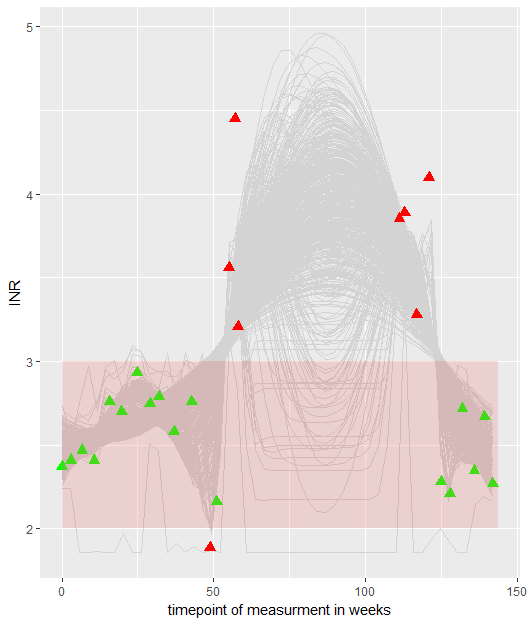
\includegraphics{./images/overlaid_gp_plots.png}
    	\label{overlaid_gp_plots}
    \end{figure}
	
	\clearpage
	
	\section{Appendix}
	\bibliography{list_of_references}
	
	\section*{Abbreviations}
	\begin{acronym}
	\acro {FIM} {Fisher Information Matrix}
	\acro {GP} {Gaussian Process}
	\acro {INR} {International normalised ratio}
	\acro {ML} {Maximum Likelihood}
	\acro {PINRR} {Percantage of INRs within the therapeutic Range}
	\acro {TTR} {Time in therapeutic range}
	\acro {VKA} {Vitamin K antagonists}
\end{acronym}



	
\end{document}